% ============================================================
%  Lumina-SN Research Proposal  (extended w/ Quantum module)
%  Juhan Kim  -- KIAS, Center for Advanced Computation
%  Compile: pdflatex (run twice for refs)
% ============================================================
\documentclass[11pt]{article}

\usepackage[T1]{fontenc}
\usepackage[utf8]{inputenc}
\usepackage[default,semibold]{sourcesanspro}
\usepackage{amsmath,amssymb}
\usepackage[a4paper,margin=2.0cm,top=1.9cm,bottom=2.0cm]{geometry}
\usepackage{graphicx}
\usepackage{xcolor}
\usepackage{titlesec}
\usepackage{enumitem}
\usepackage{booktabs}
\usepackage{array}
\usepackage{tikz}
\usepackage[most]{tcolorbox}
\usepackage{fancyhdr}
\usepackage{microtype}
\usepackage[hidelinks]{hyperref}
\usetikzlibrary{positioning,arrows.meta,backgrounds,fit,shapes.geometric}

% ---------- palette ----------
\definecolor{inkblue}{HTML}{0E2A47}
\definecolor{stellar}{HTML}{1C6FB0}
\definecolor{cyanacc}{HTML}{1496B8}
\definecolor{quantum}{HTML}{7A3FB0}
\definecolor{gold}{HTML}{C8881E}
\definecolor{ember}{HTML}{C2542E}
\definecolor{paleblue}{HTML}{EAF2FA}
\definecolor{palecyan}{HTML}{E3F3F8}
\definecolor{palequant}{HTML}{F2EBFA}
\definecolor{palegold}{HTML}{FAF1DD}
\definecolor{palegreen}{HTML}{E7F5EC}
\definecolor{darktext}{HTML}{1A1A2E}
\definecolor{rulegrey}{HTML}{C7D2DE}
\color{darktext}

% ---------- section styling ----------
\titleformat{\section}
  {\Large\bfseries\color{inkblue}}{\color{cyanacc}\thesection}{0.7em}{}
  [{\vspace{1pt}\color{cyanacc}\titlerule[1.6pt]}]
\titleformat{\subsection}
  {\large\bfseries\color{stellar}}{\color{cyanacc}\thesubsection}{0.6em}{}
\titlespacing*{\section}{0pt}{14pt}{6pt}
\titlespacing*{\subsection}{0pt}{10pt}{4pt}

% ---------- header / footer ----------
\pagestyle{fancy}\fancyhf{}
\renewcommand{\headrulewidth}{0.4pt}
\renewcommand{\footrulewidth}{0pt}
\fancyhead[L]{\footnotesize\color{stellar}\textbf{Lumina-SN}\,\textcolor{rulegrey}{|}\, Spectroscopic Dissection of SNe\,Ia}
\fancyhead[R]{\footnotesize\color{inkblue} Juhan Kim \,\textcolor{rulegrey}{|}\, KIAS}
\fancyfoot[C]{\footnotesize\color{rulegrey}\rule{0.5\linewidth}{0.4pt}}
\fancyfoot[R]{\footnotesize\color{stellar}\thepage}

% ---------- callout boxes ----------
\newtcolorbox{keybox}[1][Key Question]{breakable,enhanced,sharp corners=downhill,
  colback=palecyan,colframe=cyanacc,coltitle=white,fonttitle=\bfseries\small,
  title=#1,boxrule=0pt,leftrule=3pt,arc=1pt,left=8pt,right=8pt,top=5pt,bottom=5pt,
  attach boxed title to top left={xshift=6pt,yshift=-2pt},
  boxed title style={colback=cyanacc,arc=1pt}}
\newtcolorbox{appbox}[1][Application]{breakable,enhanced,
  colback=paleblue,colframe=stellar,coltitle=white,fonttitle=\bfseries\small,
  title=#1,boxrule=0pt,leftrule=3pt,arc=1pt,left=8pt,right=8pt,top=5pt,bottom=5pt,
  attach boxed title to top left={xshift=6pt,yshift=-2pt},
  boxed title style={colback=stellar,arc=1pt}}
\newtcolorbox{qbox}[1][Quantum Application]{breakable,enhanced,
  colback=palequant,colframe=quantum,coltitle=white,fonttitle=\bfseries\small,
  title=#1,boxrule=0pt,leftrule=3pt,arc=1pt,left=8pt,right=8pt,top=5pt,bottom=5pt,
  attach boxed title to top left={xshift=6pt,yshift=-2pt},
  boxed title style={colback=quantum,arc=1pt}}
\newtcolorbox{cautionbox}{breakable,enhanced,
  colback=palegold,colframe=gold,boxrule=0pt,leftrule=3pt,arc=1pt,
  left=8pt,right=8pt,top=5pt,bottom=5pt}

% pillar chip
\newcommand{\pillar}[3]{%
  \begin{tcolorbox}[enhanced,colback=#3,colframe=#2,boxrule=0pt,leftrule=3pt,
    arc=1pt,left=6pt,right=6pt,top=4pt,bottom=4pt,width=\linewidth]
  \textbf{\color{#2}#1}\end{tcolorbox}}

\newcommand{\code}[1]{{\small\ttfamily\color{inkblue}#1}}
\setlist[itemize]{leftmargin=1.3em,itemsep=2pt,topsep=3pt}
\setlength{\parindent}{0pt}\setlength{\parskip}{4pt}
\renewcommand{\arraystretch}{1.25}

% ============================================================
\begin{document}
\thispagestyle{empty}

% ----------------- TITLE BANNER -----------------
\begin{tikzpicture}[remember picture,overlay]
  \fill[inkblue] ([yshift=0pt]current page.north west) rectangle ([yshift=-5.4cm]current page.north east);
  \fill[cyanacc] ([yshift=-5.4cm]current page.north west) rectangle ([yshift=-5.62cm]current page.north east);
  % subtle quantum/star dots
  \foreach \x/\y in {1.3/-1.1, 3.0/-2.4, 5.1/-0.8, 7.2/-2.0, 9.0/-1.3, 11.4/-2.7, 13.0/-1.0, 15.2/-2.2, 17.6/-1.6, 19.0/-3.0, 2.2/-3.6, 6.0/-4.0, 10.0/-3.7, 14.0/-4.1, 18.0/-3.8}{
     \fill[white,opacity=0.13] ([xshift=\x cm,yshift=\y cm]current page.north west) circle (1.6pt);}
\end{tikzpicture}

\vspace{0.2cm}
{\color{white}\fontsize{12}{14}\selectfont\bfseries RESEARCH PROPOSAL}\\[2pt]
{\color{white}\fontsize{23}{27}\selectfont\bfseries Spectroscopic Dissection of Type\,Ia Supernovae}\\[5pt]
{\color{palecyan}\fontsize{15}{18}\selectfont\bfseries for Precision Cosmological Distance Measurements}\\[8pt]
{\color{palecyan}\itshape\large Toward Resolving the $H_0$ Tension and Constraining Dark Energy Evolution,\\[1pt]
grounded in first-principles, quantum-accelerated explosion physics}

\vspace{1.7cm}

{\large\bfseries\color{inkblue} Juhan Kim}\\[2pt]
{\color{darktext} Research Professor, Center for Advanced Computation}\\
{\color{darktext} Korea Institute for Advanced Study (KIAS)}\\[2pt]
{\color{stellar} February 2026 \;\textcolor{rulegrey}{\textbar}\; Revision: Quantum-Accelerated Explosion-Physics Module}

\vspace{0.5cm}

\begin{tcolorbox}[enhanced,colback=paleblue,colframe=stellar,boxrule=0pt,leftrule=4pt,
  arc=1pt,left=10pt,right=10pt,top=8pt,bottom=8pt]
{\bfseries\color{inkblue}Executive Summary.}\;
Type\,Ia supernovae (SNe\,Ia) are the cornerstone of cosmological distance measurement, yet the
empirical \emph{Phillips relation} used to standardize their luminosities may conceal physically
distinct subclasses with systematically different intrinsic brightnesses. Recent observations of
``optical twins''---SN\,Ia pairs with nearly identical optical spectra but discrepant distance
moduli---support this hypothesis, with their divergence traced to differences in near-ultraviolet
(NUV) luminosity. This proposal will (1)~develop a GPU-accelerated spectral-analysis framework
(\textbf{Lumina-SN}/\textbf{Lumina-ML}) to extract the physical parameters of SNe\,Ia from their
spectra; (2)~identify and characterize NUV-divergent subclasses with the upcoming \textbf{S-Drift}
space-UV survey; (3)~construct a refined, subclass-aware absolute-luminosity calibration that
improves $H_0$ and dark-energy constraints; and (4)~\textbf{ground the subclass physics in a
first-principles, quantum-accelerated explosion-physics module}, in which \textbf{IonQ}
(gate-model) and \textbf{D-Wave} (annealer) quantum processors attack the two computationally
hardest pieces of the deflagration-to-detonation transition (DDT)---the nuclear reaction
microphysics and the combinatorial ignition / inverse problems---that ultimately set the
$^{56}$Ni mass and iron-group distribution responsible for the observed subclasses.
\end{tcolorbox}

\vfill
{\footnotesize\color{rulegrey}\href{https://github.com/kjhan0606/Lumina-sn}{\color{stellar}github.com/kjhan0606/Lumina-sn} \;\textbar\; Lumina-SN C/CUDA Monte-Carlo radiative-transfer code}
\clearpage

% ============================================================
\section{Scientific Background and Motivation}

\subsection{Type\,Ia Supernovae as Standardizable Candles}
Type\,Ia supernovae arise from the thermonuclear disruption of carbon--oxygen white dwarfs in
binary systems. Their utility in cosmology stems from the Phillips relation (Phillips 1993): the
peak luminosity of an SN\,Ia correlates with the rate at which its light curve declines,
parameterized by $\Delta m_{15}(B)$, the $B$-band magnitude drop in the first 15 days after
maximum. This single-parameter correction transforms SNe\,Ia into standardizable candles, enabling
precise distances across cosmological scales.

The application of this relation led to the landmark discovery of cosmic acceleration (Riess
et~al.\ 1998; Perlmutter et~al.\ 1999), establishing dark energy as a central problem in modern
physics. Current SN\,Ia distances reach $\sim$5--7\% statistical precision per object after
standardization. However, as Rubin/LSST and Roman aim to constrain the dark-energy equation of
state to percent-level precision, the \emph{systematic} floor of the Phillips relation itself
becomes the limiting factor.

\begin{keybox}[Key Question]
Is the Phillips relation a single, universal relation, or does it conceal physically distinct
subclasses of SNe\,Ia with systematically different luminosity calibrations?
\end{keybox}

\subsection{The Subclass Hypothesis: Cracks in the Phillips Relation}
Mounting evidence suggests the Phillips relation may not describe a single physical sequence:
\begin{itemize}
\item \textbf{Progenitor-channel diversity:} single-degenerate (accretion) and double-degenerate
(WD merger) channels may yield subtly different nucleosynthetic yields and spectral properties even
at fixed light-curve shape.
\item \textbf{Residual Hubble scatter:} after Phillips and color corrections, the residual
scatter ($\sigma\approx0.10$--$0.15$ mag) exceeds photometric errors, implying intrinsic diversity
uncaptured by current parameters.
\item \textbf{Spectroscopic diversity:} the Wang et~al.\ (2009) split into ``Normal,''
``High-Velocity'' (HV), and 91T/91bg-like groups (via Si\,\textsc{ii} $\lambda6355$ velocity) shows
distinct populations within the ``normal'' class; HV events prefer massive hosts and may have
different Hubble residuals.
\end{itemize}

\subsection{Optical Twins and NUV Divergence: A Smoking Gun}
\begin{keybox}[Observational Evidence]
``Optical twins''---SN\,Ia pairs with nearly identical optical spectra (3500--7500\,\AA) but
measurably different distance moduli---have been identified. Crucially, these twins diverge in their
\emph{near-ultraviolet} (NUV; 2000--3500\,\AA) luminosity, indicating that the NUV carries
independent information about the explosion physics not encoded in the optical.
\end{keybox}

The striking example is SN\,2011fe and SN\,2011by (Foley \& Kirshner 2013; Graham et~al.\ 2015):
near-identical optical spectra, $\Delta m_{15}$, and colors, yet SN\,2011by was $\sim$0.335\,mag
fainter at peak in all optical bands. HST UV spectroscopy revealed dramatic divergence below
$\sim$3500\,\AA, with SN\,2011by showing suppressed NUV flux (Figure~\ref{fig:twins}). Foley \&
Kirshner attributed this to a factor $\sim$1.7 difference in $^{56}$Ni mass, though Graham et~al.\
found near-identical nebular spectra, suggesting progenitor metallicity or iron-group distribution
rather than total $^{56}$Ni mass alone.

Milne et~al.\ (2013, 2015) used Swift/UVOT to show normal SNe\,Ia separate into NUV-red and
NUV-blue subgroups (the latter $\sim$1/3 of the sample), offset by $\sim$0.4\,mag in NUV--optical
color; the NUV-blue group shows less iron-peak absorption and unburned carbon. Burns et~al.\ (2020)
studied ``sibling'' SNe in NGC\,5643 (an ideal controlled comparison), and Riess et~al.\ (2024)
demonstrated spectroscopic twins toward a precise $H_0$.

\begin{figure}[t]\centering
  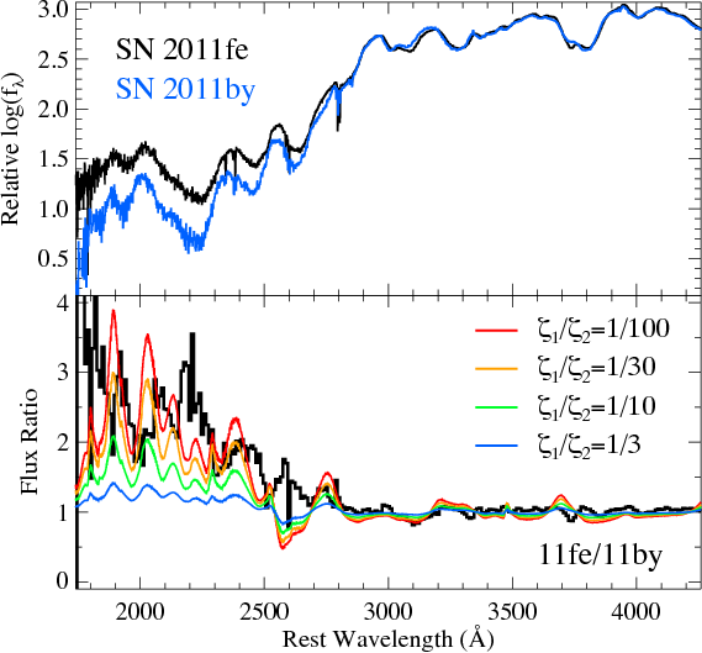
\includegraphics[width=0.66\linewidth]{fig/fig1_uvtwins.png}
  \caption{\small UV--optical spectra of the optical twins SN\,2011fe (black) and SN\,2011by (blue).
  \emph{Top:} near-identical at optical wavelengths ($\lambda>3500$\,\AA) but dramatically divergent
  in the NUV. \emph{Bottom:} flux ratio (11fe/11by); colored curves show progenitor-metallicity
  predictions $\zeta_1/\zeta_2$ (Lentz et~al.\ 2000). The NUV encodes the broken degeneracy.
  (After Graham et~al.\ 2015, MNRAS 446, 2073.)}
  \label{fig:twins}
\end{figure}

The NUV ($\lambda\lesssim3500$\,\AA) is dominated by a dense forest of iron-group element (IGE)
lines---Fe\,\textsc{ii}, Fe\,\textsc{iii}, Co\,\textsc{ii}, Ni\,\textsc{ii}---highly sensitive to:
(1)~the total $^{56}$Ni mass (which sets the peak luminosity via $^{56}$Ni\,$\to^{56}$Co\,$\to^{56}$Fe);
(2)~the \emph{radial distribution} of IGE in the ejecta (which sets the opacity structure and the
emergent UV flux); and (3)~the progenitor metallicity (which fixes the initial abundance of stable
iron-peak species, e.g.\ $^{54}$Fe, $^{58}$Ni, that blanket the UV without changing the radioactive
budget). Two SNe\,Ia can thus share an optical spectrum (set by Si, S in the outer ejecta) while
differing in NUV flux (set by IGE in the inner ejecta). \emph{The NUV flux ratio between optical
twins encodes precisely the information needed to break the luminosity degeneracy.}

% ============================================================
\section{Proposed Research Program}
This program connects theoretical spectral modeling, observational NUV surveys, cosmological
distance measurement, and---newly---a first-principles, quantum-accelerated explosion-physics module
that grounds the empirical subclass calibration in the underlying nuclear and combustion physics.

\vspace{2pt}
\pillar{Pillar~I \;\textbar\; Spectral Analysis with Lumina-SN / Lumina-ML}{stellar}{paleblue}
\pillar{Pillar~II \;\textbar\; NUV Observations with S-Drift}{cyanacc}{palecyan}
\pillar{Pillar~III \;\textbar\; Refined Absolute Luminosity \& the Hubble Law}{gold}{palegold}
\pillar{Pillar~IV \;\textbar\; Quantum-Accelerated Explosion Physics (DDT Module)}{quantum}{palequant}

\subsection{Pillar I: GPU-Accelerated Spectral Analysis}
Two codes I have developed anchor this pillar: \textbf{Lumina-SN}, a C/CUDA Monte-Carlo radiative
transfer code, and \textbf{Lumina-ML}, a neural spectral-emulation and Bayesian-inference framework.

\textbf{Lumina-SN (the forward model)} solves 1D Monte-Carlo radiative transfer in homologously
expanding ejecta under the Sobolev approximation: photon-packet emission from a sharp photosphere at
$v_{\rm ph}$, propagation through radial shells with a broken power-law density profile, and
interactions via Thomson scattering and bound--bound (Sobolev) line opacity; iterative convergence
of the radiation field ($W$, $T_{\rm rad}$) with an LTE plasma state over 5--20 cycles; and a
three-zone (Core/Wall/Outer) ejecta structure with tunable density exponents and composition (Si,
Fe, O, C, Ca, S, Mg, Ni). The C/CUDA implementation achieves $\sim$10$\times$ speedup over TARDIS on
NVIDIA GPUs, enabling the $10^4$--$10^5$ forward models required for inference.

\textbf{Lumina-ML (neural emulation \& inference).} A single Lumina-SN evaluation costs $\sim$1\,s;
to enable full Bayesian inference over a 15-D parameter space, Lumina-ML builds a neural emulator:
(1)~$5\times10^4$ spectra on a Latin-hypercube design; (2)~PCA compression of each spectrum
($\sim$1100 bins $\to\sim$60 components, $>$99.9\% variance); (3)~an MLP ($15\to60$, $\sim$500\,K
params, SiLU) mapping parameters to PCA coefficients in $\sim$10\,$\mu$s---five orders of magnitude
faster than the simulation; and (4)~inference via MCMC (\code{emcee}), nested sampling
(\code{dynesty}), and simulation-based inference (SBI/SNPE).

\begin{appbox}[Application to the Twin Problem]
Given an observed SN\,Ia spectrum, Lumina-ML returns the full posterior over 15 physical
parameters. For a twin pair we quantify exactly which parameters differ---total $^{56}$Ni mass,
iron-group distribution, or progenitor metallicity---providing the physical diagnosis that
underpins an improved luminosity calibration.
\end{appbox}

\subsection{Pillar II: NUV Observations with S-Drift}
The NUV (2000--3500\,\AA) is inaccessible from the ground, requiring space-based observation. The
\textbf{S-Drift} UV space telescope provides an ideal platform. The observational program will:
obtain NUV photometry ($\sim$2500\,\AA) and low-resolution spectroscopy for a volume-limited sample
($z<0.05$) from ZTF / Rubin-LSST; identify optical-twin pairs and measure their NUV flux ratios;
construct the first statistically significant NUV--optical color--luminosity relation; and
cross-correlate NUV properties with host-galaxy mass, metallicity, and star-formation rate to test
the progenitor-metallicity hypothesis.

\subsection{Pillar III: Refined Absolute Luminosity and the Hubble Law}
The goal is a subclass-aware calibration that replaces the single Phillips relation with a
multi-parameter standardization incorporating NUV information:
\begin{equation}
M_B = M_0 + \alpha\,(\Delta m_{15}-1.1) + \beta\,(B-V)_{\max} + \gamma\,\Delta\mathrm{NUV} + \delta\,\theta_{\rm Fe},
\end{equation}
where $\Delta$NUV is the NUV color excess (from S-Drift) and $\theta_{\rm Fe}$ is the iron-group
parameter from Lumina-ML fitting. Adding these two parameters is expected to reduce the Hubble
residual scatter from $\sigma\approx0.12$\,mag to $\sigma\lesssim0.08$\,mag---a $\sim$30\%
improvement in per-object distance precision---directly tightening $H_0$ and $w(z)$.

% ============================================================
\section{Pillar IV: Quantum-Accelerated Explosion Physics}
The empirical subclass calibration (Pillars I--III) is most powerful when grounded in the
\emph{physics that creates the subclasses}. The deflagration-to-detonation transition (DDT) in the
Chandrasekhar-mass channel sets the transition density $\rho_{\rm DDT}$, the synthesized $^{56}$Ni
mass, and the radial IGE distribution---precisely the quantities that drive the NUV divergence of
optical twins. Two pieces of the DDT problem are computationally dominant and map naturally onto the
\emph{two distinct quantum architectures} now available to this program: \textbf{IonQ} (trapped-ion
gate model) and \textbf{D-Wave} (quantum annealer).

\begin{cautionbox}
\textbf{Framing.} Pillar~IV is deliberately scoped as a \emph{NISQ-era methods-and-feasibility
thrust}, not a claim of near-term quantum advantage or near-term astrophysical constraints on $H_0$.
Each quantum workflow is paired with a strong classical baseline and judged by reusable deliverables
(QUBO formulations, benchmark datasets, sensitivity studies) and by its impact on Lumina-SN
calibration products. The same surrogate / QUBO pipelines remain scientifically useful as classical
tools should the quantum hardware underperform---an explicit fallback that de-risks the pillar.
\end{cautionbox}

\subsection{Two Architectures, Cleanly Separated}
\begin{center}
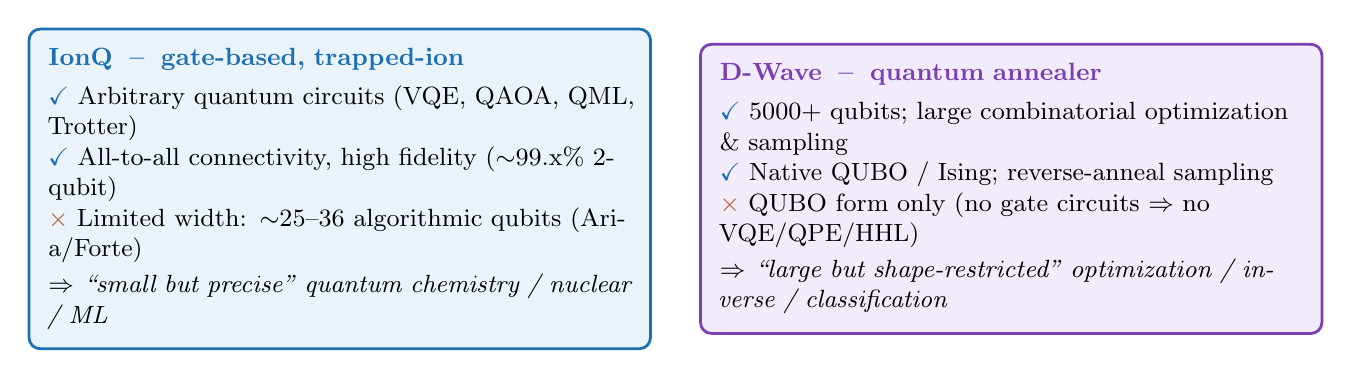
\begin{tikzpicture}[font=\small,node distance=4mm]
\node[rounded corners,draw=stellar,line width=1pt,fill=paleblue,inner sep=7pt,
      text width=7.4cm,align=left] (ionq) {%
  {\bfseries\color{stellar} IonQ \;--\; gate-based, trapped-ion}\\[3pt]
  \textcolor{stellar}{$\checkmark$} Arbitrary quantum circuits (VQE, QAOA, QML, Trotter)\\
  \textcolor{stellar}{$\checkmark$} All-to-all connectivity, high fidelity ($\sim$99.x\% 2-qubit)\\
  \textcolor{ember}{$\times$} Limited width: $\sim$25--36 algorithmic qubits (Aria/Forte)\\[2pt]
  \emph{$\Rightarrow$ ``small but precise'' quantum chemistry / nuclear / ML}};
\node[rounded corners,draw=quantum,line width=1pt,fill=palequant,inner sep=7pt,
      text width=7.4cm,align=left,right=6mm of ionq] (dwave) {%
  {\bfseries\color{quantum} D-Wave \;--\; quantum annealer}\\[3pt]
  \textcolor{stellar}{$\checkmark$} 5000+ qubits; large combinatorial optimization \& sampling\\
  \textcolor{stellar}{$\checkmark$} Native QUBO / Ising; reverse-anneal sampling\\
  \textcolor{ember}{$\times$} QUBO form only (no gate circuits $\Rightarrow$ no VQE/QPE/HHL)\\[2pt]
  \emph{$\Rightarrow$ ``large but shape-restricted'' optimization / inverse / classification}};
\end{tikzpicture}
\end{center}

\begin{keybox}[Guiding Principle]
DDT \emph{microphysics} (nuclear reaction rates) $\rightarrow$ \textbf{IonQ}. \quad
DDT \emph{combinatorial \& inverse problems} (ignition placement, parameter estimation)
$\rightarrow$ \textbf{D-Wave}. \;Do not mix the roles.
\end{keybox}

\subsection{D-Wave: The Combinatorial \& Inverse Half of the DDT}

\subsubsection*{IV.1\quad Multi-Spot Ignition-Kernel Placement via a Quadratic Surrogate}
In DDT-class models the initial deflagration ignition geometry---how many kernels to seed, and where
in the white-dwarf core---governs the $^{56}$Ni mass and its radial distribution, and hence the
light curve and NUV color. This is a \emph{combinatorial placement} problem over binary occupation
variables $x_i\in\{0,1\}$ (kernel at a physics-filtered candidate site $i$). The full radiation-hydro
response $L_\lambda(\mathbf{x})$ is nonlinear in $\mathbf{x}$ and is \emph{not} directly a QUBO; we
therefore fit a \emph{quadratic response surrogate} over the candidate sites,
\begin{equation}
L_\lambda^{\rm model}(\mathbf{x}) \;\approx\; L_\lambda^{0} + \sum_i a_{\lambda i}\,x_i
   + \sum_{i<j} b_{\lambda ij}\,x_i x_j ,
\end{equation}
with coefficients learned from a designed ensemble of classical 1D/2D explosion models. The resulting
objective $\sum_\lambda(L_\lambda^{\rm obs}-L_\lambda^{\rm model})^2 + \lambda_1(\sum_i x_i-N_k)^2 +
\lambda_2\sum_{\langle ij\rangle}J_{ij}x_i x_j$ (count and minimum-separation penalties) is then an
explicit QUBO. The D-Wave annealer \emph{samples low-energy configurations} of this quadratic
approximation inside an \emph{outer classical loop} that updates the surrogate and validates
candidate placements with full Lumina-SN evaluations.

\begin{qbox}[Most actionable near-term use case]
Surrogate-based ignition placement is the most actionable near-term quantum-hardware task in this
program. Because quantum annealers have not demonstrated a general optimization advantage for this
problem class, \emph{all} D-Wave results will be benchmarked on identical surrogate objectives
against strong classical methods---simulated annealing, parallel tempering, tabu search, Bayesian
optimization, and (where tractable) exact / mixed-integer quadratic optimization---with success
measured by solution quality, time-to-target, and solution diversity.
\end{qbox}

\subsubsection*{IV.2\quad DDT-Parameter Inverse Estimation}
Continuous DDT parameters---the transition density $\rho_{\rm DDT}$, the Karlovitz-number threshold,
etc.---are recovered by binary expansion into QUBO variables and minimizing the model--observation
(spectrum / light-curve) mismatch. Reverse annealing is used as an \emph{approximate local sampler /
proposal generator} for this multimodal inverse problem---\emph{not} assumed to be a calibrated
Bayesian posterior; posterior claims are made only after validation against classical
MCMC / nested-sampling baselines on test problems with known targets, before combining with ZTF/LSST
ensemble statistics.

\subsubsection*{IV.3\quad QBoost --- a DDT-Precursor Classifier}
Using existing 3D explosion simulations as labelled training data, a classifier for ``where DDT
ignites'' is learned with D-Wave \textbf{QBoost} (sparse weak-learner ensemble selection cast as a
QUBO), benchmarked against logistic regression, random forests, and gradient boosting (XGBoost) under
class imbalance (AUROC/AUPRC, false-positive rate at fixed recall). The QUBO's sparse learner
selection is valued for \emph{interpretability} of the precursor indicators, not assumed accuracy
advantage.

\subsection{IonQ: The Nuclear-Microphysics Half of the DDT}

\subsubsection*{IV.4\quad VQE --- Restricted Nuclear-Structure Benchmark for the DDT Chain}
The DDT density $\rho_{\rm DDT}$ depends on the induction-time gradient (Zel'dovich gradient
mechanism), and $\tau_{\rm ind}$ is strongly temperature- and rate-sensitive to the $^{12}$C$+^{12}$C
reaction. We scope the IonQ task \emph{honestly}: a VQE on 25--36 noisy qubits cannot produce a
predictive $^{12}$C$+^{12}$C astrophysical $S$-factor (a sub-barrier fusion problem involving
tunneling, resonances, compound-$^{24}$Mg states, channel couplings, and partial widths). Instead,
VQE will target a \emph{restricted active-space shell-model Hamiltonian} for selected $^{24}$Mg
levels (Jordan--Wigner mapping; IonQ's all-to-all connectivity suits the dense nuclear term
structure), benchmarked against \emph{exact diagonalization} in the same truncated space. The
physically meaningful chain is therefore:
\[
\text{VQE restricted spectrum} \;\to\; \text{benchmarked level-energy sensitivity}
\;\to\; \text{perturbation of a conventional reaction-rate model} \;\to\; \text{propagated } \tau_{\rm ind}\text{ sensitivity},
\]
\emph{not} a standalone quantum prediction of the rate.

\begin{qbox}[Deliverable]
A demonstrated workflow propagating controlled nuclear-Hamiltonian perturbations into $\tau_{\rm
ind}$ \emph{sensitivity} (``if a level/rate shifts by $X\%$, the DDT criterion moves by $\dots$''),
anchored to established classical reaction-rate calculations---a sensitivity-informed correction, not
a production $\tau_{\rm ind}(\rho,T,X)$ table. This preserves the link to the Zel'dovich mechanism
while remaining honest about NISQ and model-space limitations.
\end{qbox}

\subsubsection*{IV.5\quad Variational Quantum Classifier (QML)}
A variational quantum classifier (VQC) learns DDT-precursor patterns as a \emph{diagnostic benchmark}
against the D-Wave QBoost classifier (IV.3) and classical ML---a publishable annealer-vs-gate study.
On small noisy devices a VQC is not expected to beat classical ML on tabular data; its value is the
controlled cross-architecture comparison, not a flagship accuracy claim.

\subsubsection*{IV.6\quad QAOA --- Small-Scale Ignition Placement (annealer benchmark)}
The same ignition-placement QUBO (IV.1) solved on IonQ via \textbf{QAOA} provides a direct
\emph{annealer-vs-gate} performance comparison---a methodology contribution in its own right.

\subsection{Hybrid Integration with the Classical SN\,Ia Code}
\begin{center}
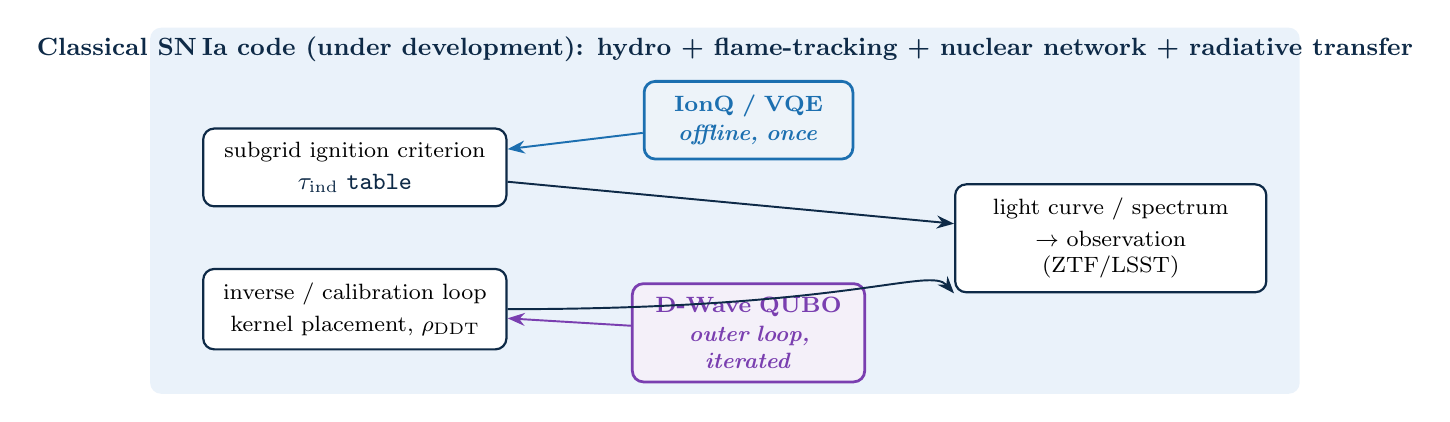
\begin{tikzpicture}[font=\footnotesize,node distance=5mm,
  block/.style={rounded corners,draw=inkblue,line width=0.8pt,fill=white,inner sep=5pt,align=center},
  qchip/.style={rounded corners,draw=#1,line width=1pt,fill=#1!8,inner sep=5pt,align=center,text=#1},
  ar/.style={-{Stealth[length=2.2mm]},line width=0.7pt}]
\begin{scope}[on background layer]
 \node[rounded corners,fill=paleblue,minimum width=14.6cm,minimum height=4.65cm] (bg) {};
\end{scope}
\node[anchor=north,text=inkblue,font=\bfseries\small] at (bg.north) {Classical SN\,Ia code (under development): hydro + flame-tracking + nuclear network + radiative transfer};
\node[block,text width=3.5cm] (ign) at (-4.7,0.55) {subgrid ignition criterion\\[2pt]\code{$\tau_{\rm ind}$ table}};
\node[block,text width=3.5cm] (cal) at (-4.7,-1.25) {inverse / calibration loop\\[2pt]kernel placement, $\rho_{\rm DDT}$};
\node[block,text width=3.6cm] (out) at (4.9,-0.35) {light curve / spectrum\\[2pt]$\rightarrow$ observation (ZTF/LSST)};
\node[qchip=stellar,text width=2.3cm] (ionq) at (0.3,1.15) {\bfseries IonQ / VQE\\[1pt]\itshape offline, once};
\node[qchip=quantum,text width=2.6cm] (dwave) at (0.3,-1.55) {\bfseries D-Wave QUBO\\[1pt]\itshape outer loop, iterated};
\draw[ar,stellar] (ionq) -- (ign);
\draw[ar,quantum] (dwave) -- (cal);
\draw[ar,inkblue] (ign) -- (out);
\draw[ar,inkblue] (cal.east) .. controls (1.6,-1.25) and (2.6,-0.7) .. (out.south west);
\end{tikzpicture}
\end{center}
\vspace{-2pt}
\begin{itemize}
\item \textbf{IonQ output $=$ offline lookup table:} per-timestep quantum calls are infeasible
(latency, queueing); reaction rates / $\tau_{\rm ind}$ are precomputed and tabulated into the code.
\item \textbf{D-Wave output $=$ external calibration loop:} the explosion simulation is wrapped in a
surrogate, and the annealer searches parameters / ignition placement around it.
\end{itemize}

\subsection{Minimum-Viable Starting Projects}
\begin{center}\small
\begin{tabular}{@{}p{0.49\linewidth} p{0.49\linewidth}@{}}
\toprule
\textbf{\color{quantum}Project A --- D-Wave} (recommended first; faster results) &
\textbf{\color{stellar}Project B --- IonQ} \\
\midrule
\emph{Optimize multi-spot ignition placement (quadratic surrogate) to match an observed light curve.} &
\emph{VQE benchmark of a restricted $^{24}$Mg active-space spectrum.} \\[3pt]
1.\ Build a placement\,$\to$\,light-curve quadratic surrogate from 1D/2D models.\newline
2.\ Encode the surrogate mismatch as a QUBO.\newline
3.\ Submit via the Ocean SDK (\code{dwave-system}, \code{dimod}).\newline
4.\ Benchmark vs.\ simulated annealing / parallel tempering. &
1.\ Select a small active-space shell-model Hamiltonian.\newline
2.\ Build the VQE (Qiskit-Nature / PennyLane).\newline
3.\ Submit on the IonQ backend (Qiskit-IonQ / PennyLane-IonQ).\newline
4.\ Validate vs.\ exact diagonalization; simulator\,$\to$\,hardware. \\
\bottomrule
\end{tabular}
\end{center}
The Ocean SDK has a gentle learning curve, with first results expected within a few weeks.

\subsection{Evaluation, Baselines, and Resource Accounting}
Each quantum task carries a pre-registered classical baseline and quantitative success criteria, so
that ``does quantum help here?'' is answered, not assumed:
\begin{itemize}
\item \textbf{Baselines:} simulated annealing, parallel tempering, tabu search, Bayesian
optimization, and MILP/MIQP (D-Wave / QAOA); exact diagonalization and classical shell-model codes
(VQE); logistic regression, random forests, XGBoost (classifiers).
\item \textbf{Success metrics:} best objective value and time-to-target on identical surrogate
objectives; solution diversity and robustness to surrogate noise; reproducibility across anneals;
VQE energy error vs.\ exact diagonalization; AUROC/AUPRC under imbalance; and---ultimately---the
change in Lumina-SN spectral / light-curve residuals.
\item \textbf{Resource accounting:} number of binary variables, QUBO density, coefficient precision,
D-Wave minor-embedding overhead and chain-strength strategy (logical vs.\ physical qubits); for IonQ,
circuit depth, shot budgets, and measurement / symmetry-based error mitigation.
\item \textbf{Surrogate validity:} $L_\lambda^{\rm model}(\mathbf{x})$ is trained, cross-validated,
and locally re-quadratized within the outer loop, with surrogate-to-QUBO uncertainty propagated.
\end{itemize}

\subsection{Honest Caveats}
\begin{cautionbox}
\begin{itemize}
\item \textbf{D-Wave cannot run VQE/HHL.} Linear-system and reaction-network solves belong to IonQ
(or future FTQC). Keep the architectural roles separate.
\item \textbf{IonQ qubit limits} strongly constrain the nuclear model space---initial goals target
\emph{demonstrated quantum feasibility}, not yet quantitative accuracy.
\item \textbf{Quantum CFD} (direct turbulent-flame simulation) is beyond both machines---an FTQC-era
problem, deferred.
\item \textbf{Latency:} cloud-queue waits make in-line simulation calls impractical on both
platforms $\Rightarrow$ the offline-table / external-loop pattern is mandatory.
\end{itemize}
\end{cautionbox}

% ============================================================
\section{Methodology and Timeline}
\begin{center}\small
\begin{tabular}{@{}>{\raggedright\arraybackslash}p{2.05cm} >{\raggedright\arraybackslash}p{13.0cm}@{}}
\toprule
\textbf{\color{inkblue}Phase} & \textbf{\color{inkblue}Activities} \\
\midrule
\textbf{Phase 1}\newline\textit{Year 1} &
Generate $\sim$$10^5$ Lumina-SN synthetic spectra spanning the SN\,Ia parameter space (emphasis on
IGE abundance/distribution); train and validate the Lumina-ML emulator ($<$1\% RMS, 2000--10000\,\AA);
apply Bayesian inference to archival spectra (CfA/CSP/Berkeley). \textbf{Quantum kickoff:} Project~A
(D-Wave ignition-placement QUBO) and Project~B (IonQ VQE proof-of-concept) on simulators. \\
\textbf{Phase 2}\newline\textit{Year 1--2} &
Automated optical-twin identification (3800--7200\,\AA\ cross-correlation, $\sim$3000 spectra);
per-twin 15-parameter posteriors and identification of the luminosity-discrepancy driver; NUV
predictions for S-Drift. \textbf{Quantum:} D-Wave hardware runs + classical-SA benchmark; IonQ
hardware validation; $\tau_{\rm ind}$ table v1. \\
\textbf{Phase 3}\newline\textit{Year 2--3} &
S-Drift NUV photometry/spectroscopy of new SNe\,Ia and twin candidates; validate Lumina-ML
predictions; build the subclass-aware calibration (Eq.~1) and quantify the scatter improvement.
\textbf{Quantum:} couple $\tau_{\rm ind}$ corrections + ignition placement into the explosion module;
annealer-vs-gate (QAOA) comparison study. \\
\textbf{Phase 4}\newline\textit{Year 3} &
Apply the refined calibration to Pantheon+ / Union; derive updated $H_0$, $w(z)$; assess Hubble-tension
relief; prepare for Rubin/LSST and Roman. \\
\bottomrule
\end{tabular}
\end{center}

% ============================================================
\section{Technical Readiness and Resources}
\begin{itemize}
\item \textbf{Lumina-SN} is operational, validated against TARDIS to sub-1\% ($W$ error 0.44\%,
$T_{\rm rad}$ error 0.36\%), and demonstrated on SN\,2011fe (best-fit RMS $=0.0894$). The C/CUDA
build achieves $\sim$10$\times$ GPU speedup (200\,K packets: 728\,ms GPU vs.\ 7.2\,s CPU).
\item \textbf{Lumina-ML} provides a complete emulation + inference pipeline (MCMC, nested sampling,
SBI); the emulator evaluates spectra in $\sim$10\,$\mu$s.
\item \textbf{Computing:} KIAS CAC dedicated GPU clusters (NVIDIA A100/H100); additional KISTI
Nurion/Neuron allocations via the Grand Challenge Program.
\item \textbf{Quantum access:} IonQ (gate-model, via cloud providers) and D-Wave (Leap / Ocean SDK)
for Pillar~IV; both used in the offline-table / external-loop pattern above.
\item \textbf{Collaborations:} KASI supernova group, the FOSTER multi-wavelength group, and the SDSS
Korean Scientist Group for spectral databases.
\end{itemize}

% ============================================================
\begin{figure}[t]\centering
  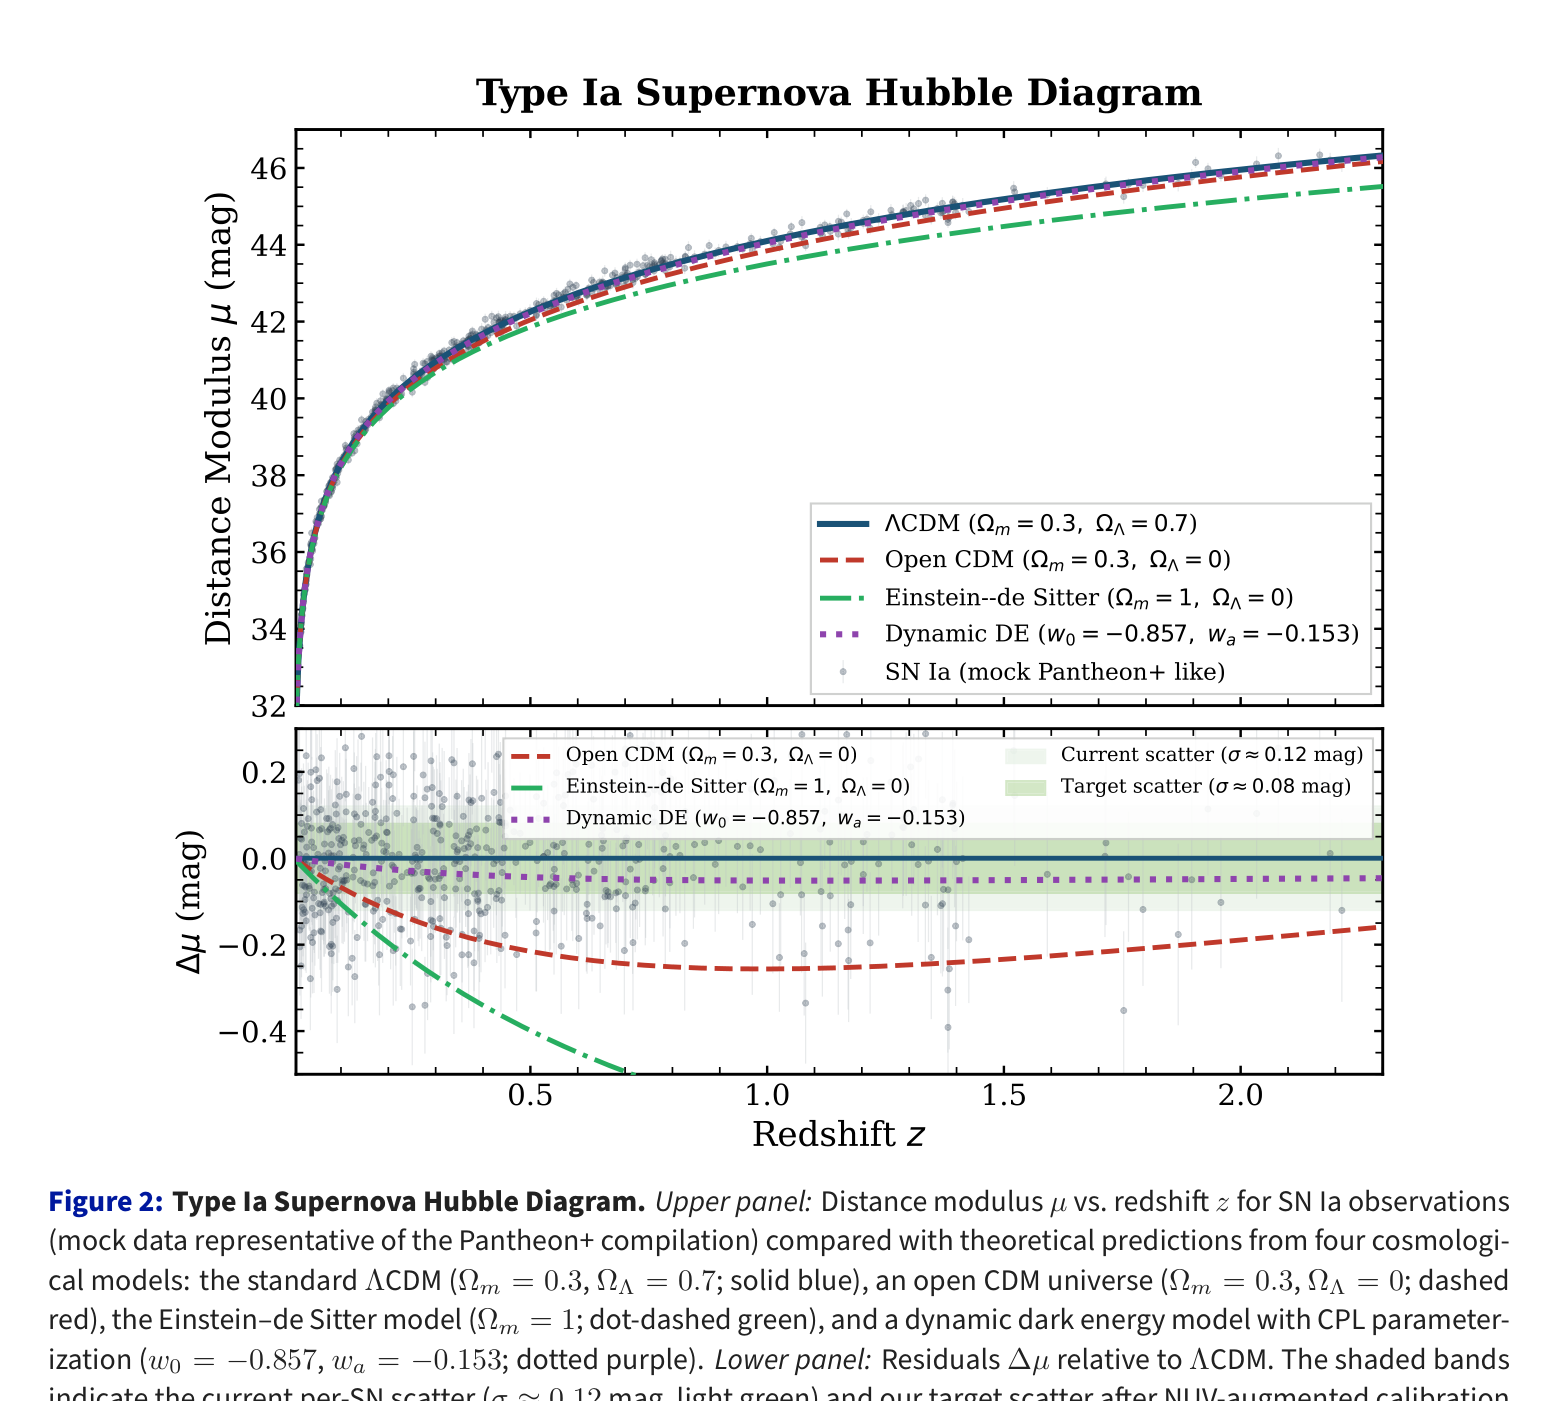
\includegraphics[width=0.88\linewidth]{fig/fig2_hubble.png}
  \caption{\small \textbf{Type\,Ia Supernova Hubble diagram.} \emph{Upper:} distance modulus vs.\
  redshift for mock Pantheon+-like data against four cosmologies ($\Lambda$CDM; open CDM;
  Einstein--de\,Sitter; CPL dynamic dark energy $w_0=-0.857$, $w_a=-0.153$). \emph{Lower:} residuals
  $\Delta\mu$ relative to $\Lambda$CDM; bands show the current per-SN scatter ($\sigma\approx0.12$
  mag) and the target after NUV-augmented calibration ($\sigma\approx0.08$). Distinguishing
  $\Lambda$CDM from dynamic dark energy requires sub-0.1-mag precision---motivating the improved
  standardization proposed here.}
  \label{fig:hubble}
\end{figure}

\section{Expected Outcomes and Impact}
\begin{enumerate}[leftmargin=1.5em]
\item \textbf{Physical classification of SN\,Ia subclasses:} the first systematic mapping between
spectroscopically inferred parameters (IGE mass/distribution, progenitor metallicity) and the
optical-twin / NUV-divergence phenomenon.
\item \textbf{NUV-augmented luminosity calibration:} a new standardization (Eq.~1) reducing Hubble
scatter by $\sim$30\% ($\sigma\approx0.12\to\lesssim0.08$\,mag).
\item \textbf{Improved $H_0$:} tighter local distance-ladder constraints bearing directly on the
Hubble tension.
\item \textbf{First-principles explosion grounding:} a quantum-accelerated DDT module linking nuclear
microphysics ($\tau_{\rm ind}$) and ignition combinatorics to the observable subclasses---plus
standalone methodology results (annealer-vs-gate; QBoost-vs-VQC).
\item \textbf{Public code release:} Lumina-SN, Lumina-ML, the trained emulator, the template library,
and the quantum-module scaffolding.
\item \textbf{S-Drift synergy:} a key science case for the S-Drift UV mission.
\end{enumerate}

% ============================================================
\section{Cosmological Applications: $H_0$ Tension and Dynamic Dark Energy}

\subsection{The Hubble Tension}
The $\sim$5$\sigma$ discrepancy between the local $H_0$ ($73.0\pm1.0$\,km/s/Mpc, SH0ES; Riess
et~al.\ 2022) and the CMB-inferred value ($67.4\pm0.5$\,km/s/Mpc, Planck 2020) remains unresolved. A
significant share of the local error budget originates in the SN\,Ia standardization step: if
unrecognized subclasses with different luminosities are mixed into the calibrator sample, $H_0$ may
be biased. Our NUV-augmented calibration will quantify whether the SH0ES calibrator sample contains
a NUV-red/NUV-blue mixture, and whether correcting it shifts $H_0$---providing a cleaner,
subclass-homogeneous distance ladder and reducing $H_0$ systematics below the current $\sim$1.4\%
level.

\subsection{Dynamic Dark Energy and the Equation of State $w(z)$}
Unrecognized astrophysical systematics in the SN\,Ia Hubble diagram can mimic or mask dynamic dark
energy. Our subclass-aware calibration removes this systematic, enabling a clean test of
$w(z)\ne-1$. Combining improved SN\,Ia distances with DESI/SDSS BAO and Planck/ACT CMB constraints,
we will construct a joint analysis simultaneously constraining $H_0$, $\Omega_m$, and the CPL
parameters $(w_0,w_a)$---the most stringent test to date of whether dark energy is a cosmological
constant or an evolving component.

\begin{tcolorbox}[enhanced,colback=inkblue,colframe=inkblue,coltext=white,boxrule=0pt,arc=2pt,
  left=10pt,right=10pt,top=8pt,bottom=8pt]
\textbf{In summary,} this proposal bridges computational spectral modeling (Lumina-SN/ML),
space-based NUV observation (S-Drift), precision cosmology, and a first-principles,
quantum-accelerated explosion-physics module (IonQ\,+\,D-Wave). By revealing and quantifying the
physical substructure hidden within the Phillips relation---and grounding it in the nuclear and
combustion physics that creates it---we aim to improve SN\,Ia distance precision by $\sim$30\%,
directly contributing to the resolution of the $H_0$ tension and to constraining the time evolution
of dark energy.
\end{tcolorbox}

\end{document}
